% ==============================================================================
% VLIZ Scientific Research Poster - IMDIS 2026: Marine Term Translations (MTT)
% ==============================================================================
% Audience: Domain Translators & Ontology / Vocabulary Maintainers
% Layout: Option 2 — Central Hero Showcase + 2x2 Flanking Persona Grid
% Branding: VLIZ Sea-Teal (#91C8CD) + Reserved IMDIS 2026 Logo & Partner Slots
% Empirical Standard: Khadka & Peeters (2024) MAR Exemplary Tier (70/30 Rule)
% ==============================================================================

\documentclass[
  25pt,
  a0paper,
  portrait,
  margin=0mm,
  innermargin=15mm,
  blockverticalspace=7mm,
  colspace=10mm,
  subcolspace=8mm
]{tikzposter}

\usepackage{graphicx}
\graphicspath{{assets/}{posters/imdis-marine-term-translations/assets/}{posters/marine-term-translations/assets/}{templates/posters/assets/}}
\usepackage{amsmath,amssymb}
\usepackage{qrcode}
\usepackage{hyperref}
\usepackage{tikz}
\usetikzlibrary{positioning,calc,arrows.meta}
\usepackage{tcolorbox}

% ------------------------------------------------------------------------------
% VLIZ Institutional Color Palette
% ------------------------------------------------------------------------------
\definecolor{vlizBanner}{HTML}{91C8CD}       % Sea-teal top banner
\definecolor{vlizTeal}{HTML}{31B7BC}         % Vibrant teal subtitle & accents
\definecolor{vlizNavy}{HTML}{3057A5}         % VLIZ Corporate Navy
\definecolor{vlizCharcoal}{HTML}{231F20}     % Dark Charcoal author text
\definecolor{vlizSlateText}{HTML}{1E293B}    % Main body text
\definecolor{vlizSlateMuted}{HTML}{64748B}   % Muted caption/affiliation text
\definecolor{vlizCardBg}{HTML}{FFFFFF}       % White card background
\definecolor{vlizHeroBg}{HTML}{F8FAFC}       % Soft slate sub-card background
\definecolor{vlizBorder}{HTML}{CBD5E1}       % Card border
\definecolor{vlizLightTeal}{HTML}{E6F7F8}   % Light teal callout background

% Set custom tikzposter style
\definecolorstyle{VLIZStyle}{
  \definecolor{colorOne}{HTML}{3057A5}
  \definecolor{colorTwo}{HTML}{31B7BC}
  \definecolor{colorThree}{HTML}{91C8CD}
}{
  \colorlet{backgroundcolor}{white}
  \colorlet{framecolor}{white}
  \colorlet{titlefgcolor}{vlizNavy}
  \colorlet{titlebgcolor}{white}
  \colorlet{blocktitlebgcolor}{white}
  \colorlet{blocktitlefgcolor}{vlizNavy}
  \colorlet{blockbodybgcolor}{vlizCardBg}
  \colorlet{blockbodyfgcolor}{vlizSlateText}
}

\usetheme{Default}
\usecolorstyle{VLIZStyle}
\tikzposterlatexaffectionproofoff

% Custom block style: Clean rounded card with crisp border
\defineblockstyle{VLIZBlock}{
  titlewidthscale=1.0, bodywidthscale=1.0,
  titleoffsetx=0pt, titleoffsety=0pt, bodyoffsetx=0pt, bodyoffsety=0pt,
  bodyverticalshift=0pt, roundedcorners=14, linewidth=2pt,
  titleinnersep=4mm, bodyinnersep=5.5mm
}{
  \draw[color=vlizBorder, fill=blockbodybgcolor, rounded corners=14, line width=2pt]
    (blockbody.south west) rectangle (blocktitle.north east);
}
\useblockstyle{VLIZBlock}

\title{}
\author{}
\institute{}

\begin{document}

% ==============================================================================
% 1. TOP BANNER (Official VLIZ Vector Header)
% ==============================================================================
\fill[vlizBanner] (-0.5\paperwidth, 0.5\paperheight)
  rectangle (0.5\paperwidth, {0.5\paperheight - 0.112\paperheight});

% Vector VLIZ Logo (Left)
\node[anchor=west, inner sep=0pt] at ({-0.5\paperwidth + 0.088\paperwidth}, {0.5\paperheight - 0.056\paperheight}) {
  
\includegraphics[height=0.064\paperheight]{vliz_logo.png}
};

% Sharp Native Vector Typography for URL (Right)
\node[anchor=east, inner sep=0pt] at ({0.5\paperwidth - 0.088\paperwidth}, {0.5\paperheight - 0.056\paperheight}) {
  {\color{vlizNavy}\sffamily\bfseries\fontsize{34pt}{40pt}\selectfont vliz.be}
};

% ==============================================================================
% 2. TITLE & AUTHORS SECTION + RESERVED IMDIS 2026 CONFERENCE LOGO SLOT
% ==============================================================================
\node[anchor=north west, text width=0.695\paperwidth, align=flush left, inner sep=0pt]
  at ({-0.5\paperwidth + 0.088\paperwidth}, {0.5\paperheight - 0.123\paperheight}) {
  % Subtitle / Venue & Audience Callout
  {\color{vlizTeal}\bfseries\Large IMDIS 2026 \quad $\vert$ \quad mtt.vliz.be \quad $\vert$ \quad FOR DOMAIN TRANSLATORS \& ONTOLOGY MAINTAINERS \par}
  \vspace{0.25cm}
  % Main Title
  {\color{vlizNavy}\bfseries\fontsize{41pt}{49pt}\selectfont Marine Term Translations (MTT): A Self-Hosted Platform for Multilingual Marine Terminology Interoperability \par}
  \vspace{0.28cm}
  % Author
  {\color{vlizCharcoal}\bfseries\LARGE Cedric Decruw \par}
  \vspace{0.16cm}
  % Affiliations & Contact
  {\color{vlizSlateMuted}\large Flanders Marine Institute (VLIZ), Ostend, Belgium \quad $\vert$ \quad cedric.decruw@vliz.be \quad $\vert$ \quad ORCID: 0000-0001-6387-5988 \par}
};

% Reserved Default Conference Logo Placeholder Box (title_header_right)
\node[anchor=north east, inner sep=0pt]
  at ({0.5\paperwidth - 15mm}, {0.5\paperheight - 0.124\paperheight}) {
  
\begin{tikzpicture}
    \node[
      draw=vlizTeal,
      dashed,
      line width=2pt,
      fill=vlizHeroBg,
      rounded corners=10,
      minimum width=12.2cm,
      minimum height=8.8cm,
      align=center
    ] {
      {\color{vlizNavy}\bfseries\Large [ IMDIS 2026 Logo ]}\\[6pt]
      {\color{vlizSlateMuted}\normalsize Reserved Conference}\\
      {\color{vlizSlateMuted}\normalsize Logo Space}
    };
  \end{tikzpicture}
};

% ==============================================================================
% Set starting vertical position for tikzposter blocks
% ==============================================================================
\makeatletter
\setlength{\TP@blocktop}{0.5\textheight - 266mm}
\makeatother

% ==============================================================================
% 3. TOP 2-COLUMN FLANKING BAND: CONTEXT/RQ & BODC P02 BETA RESULTS
% ==============================================================================
\begin{columns}
  % ---- Top-Left: Context, Research Question & Hypothesis ----
  \column{0.50}
  \block{1. Context, Research Question \& Hypothesis}{
    \textbf{Operational Gap in Marine Vocabularies:}
    \begin{itemize}\setlength{\itemsep}{2pt}
      \item Marine infrastructures (SeaDataNet, EMODnet, BODC NVS) maintain authoritative terms in English, while translations rely on disconnected spreadsheets.
      \item Periodic full-snapshot downloads cause sync lag and URI drift.
    \end{itemize}

    \vspace{0.15cm}
    \begin{tcolorbox}[colback=vlizLightTeal,colframe=vlizBanner,arc=4mm,boxrule=1.5pt,left=5mm,right=5mm,top=2.8mm,bottom=2.8mm]
      {\color{vlizNavy}\bfseries Research Question (RQ)}\\[2pt]
      {\small\textit{How can institutions run a sovereign multilingual terminology workflow that engages domain experts and publishes machine-actionable updates?}}
    \end{tcolorbox}

    \vspace{0.12cm}
    \begin{tcolorbox}[colback=vlizHeroBg,colframe=vlizBorder,arc=4mm,boxrule=1.5pt,left=5mm,right=5mm,top=2.8mm,bottom=2.8mm]
      {\color{vlizNavy}\bfseries Hypothesis \& Prediction}\\[2pt]
      {\small\textit{Decoupling persistent concept URIs from language labels in an ORCID-governed, LDES-enabled web platform eliminates sync lag without URI churn.}}
    \end{tcolorbox}
  }

  % ---- Top-Right: BODC P02 Beta Evaluation & Verdict ----
  \column{0.50}
  \block{2. Empirical Evaluation (BODC P02 Beta)}{
    \textbf{Observed Beta Performance Metrics:}
    \vspace{0.12cm}

    \noindent
    \begin{minipage}{0.32\linewidth}
      \begin{tcolorbox}[colback=vlizLightTeal,colframe=vlizNavy,arc=4mm,boxrule=2pt,halign=center,top=2.5mm,bottom=2.5mm]
        {\color{vlizNavy}\bfseries\fontsize{30pt}{34pt}\selectfont 25\%}\\[2pt]
        {\small P02 in NL \& FR}
      \end{tcolorbox}
    \end{minipage}\hfill
    \begin{minipage}{0.32\linewidth}
      \begin{tcolorbox}[colback=vlizHeroBg,colframe=vlizTeal,arc=4mm,boxrule=2pt,halign=center,top=2.5mm,bottom=2.5mm]
        {\color{vlizTeal}\bfseries\fontsize{30pt}{34pt}\selectfont 2$\times$}\\[2pt]
        {\small Drafting Speed}
      \end{tcolorbox}
    \end{minipage}\hfill
    \begin{minipage}{0.32\linewidth}
      \begin{tcolorbox}[colback=vlizLightTeal,colframe=vlizNavy,arc=4mm,boxrule=2pt,halign=center,top=2.5mm,bottom=2.5mm]
        {\color{vlizNavy}\bfseries\fontsize{30pt}{34pt}\selectfont 0}\\[2pt]
        {\small Concept URI Churn}
      \end{tcolorbox}
    \end{minipage}

    \vspace{0.15cm}
    \begin{tcolorbox}[colback=vlizLightTeal,colframe=vlizBanner,arc=4mm,boxrule=1.5pt,left=5mm,right=5mm,top=2.8mm,bottom=2.8mm]
      {\color{vlizNavy}\bfseries Live RDF Stream Continuity}\\[2pt]
      {\small Validated Dutch and French P02 concepts published immediately as an incremental LDES endpoint.}
    \end{tcolorbox}

    \vspace{0.12cm}
    \begin{tcolorbox}[colback=vlizHeroBg,colframe=vlizBorder,arc=4mm,boxrule=1.5pt,left=5mm,right=5mm,top=2.8mm,bottom=2.8mm]
      {\color{vlizNavy}\bfseries Discussion, Limitation \& Future Direction}\\[2pt]
      {\small
      $\bullet$ \textbf{Supported Hypothesis:} End-to-end LDES sync proven without URI churn.\\
      $\bullet$ \textbf{1 Study Limitation:} Review velocity bounded by domain-expert bandwidth.\\
      $\bullet$ \textbf{Future Direction:} Automated confidence triage to prioritize expert review.}
    \end{tcolorbox}
    \vspace*{12.03mm}
  }
\end{columns}

% ==============================================================================
% 4. DOMINANT CENTRAL HERO SHOWCASE (Full-Width Eye-Level Zone)
% ==============================================================================
\block{}{
  \centering
  \vspace{-0.15cm}
  {\color{vlizNavy}\bfseries\huge Central Architecture: RDF LDES Ingestion $\rightarrow$ Curated Translation $\rightarrow$ Enriched LDES $\rightarrow$ vocab.vliz.be Widget \par}
  \vspace{0.12cm}
  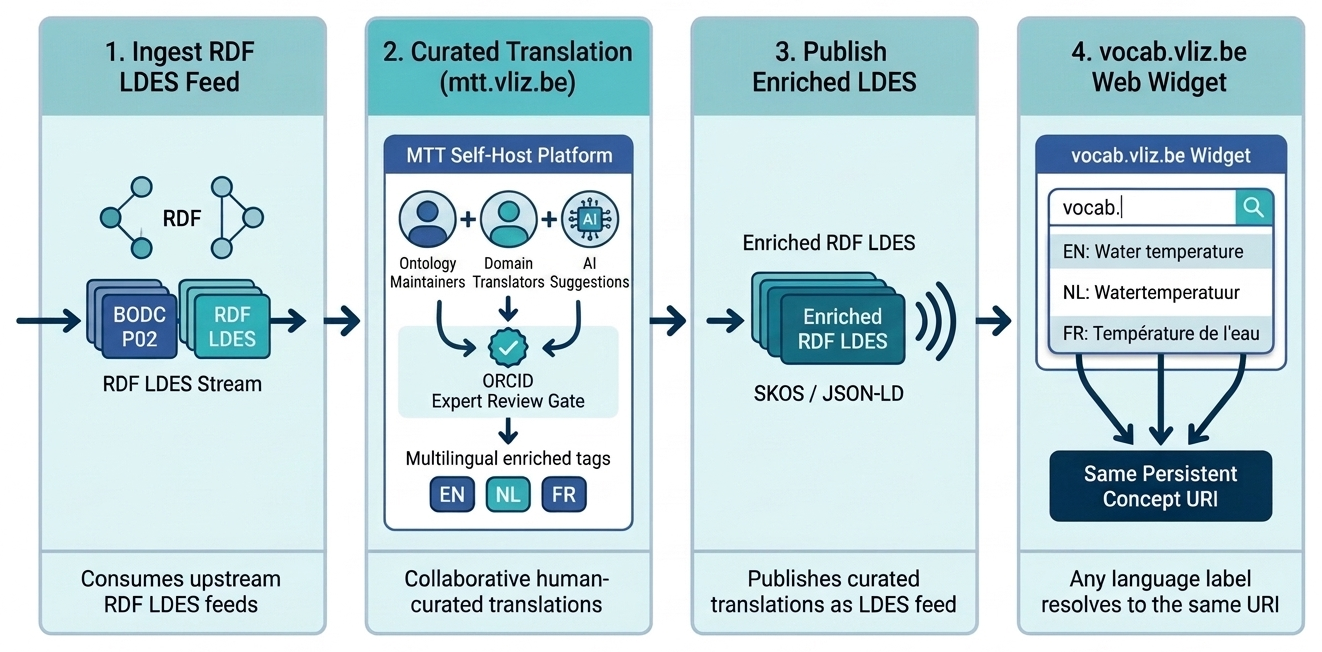
\includegraphics[width=0.96\linewidth]{imdis-mtt-ldes-hero.png}\\[-0.05cm]
  {\color{vlizSlateMuted}\large \textbf{Figure 1:} MTT consumes upstream RDF LDES streams (e.g. BODC P02), supports human-curated translations with AI drafting and ORCID review, re-publishes enriched RDF LDES feeds, and powers \texttt{vocab.vliz.be} widgets where any multilingual label resolves to the \textbf{same persistent Concept URI}.}
  \vspace{-0.1cm}
}

% ==============================================================================
% 5. BOTTOM 2-COLUMN FLANKING BAND: DUAL-PERSONA VALUE & DUAL QR ACCESS
% ==============================================================================
\begin{columns}
  % ---- Bottom-Left: For Ontology Maintainers & Domain Translators ----
  \column{0.50}
  \block{3. For Ontology Maintainers \& Domain Translators}{
    \textbf{For Ontology / Vocabulary Owners \& Maintainers:}
    \vspace{0.1cm}

    \noindent
    \begin{minipage}{0.49\linewidth}
      \begin{tcolorbox}[colback=vlizLightTeal,colframe=vlizBanner,arc=4mm,boxrule=1.5pt,left=4mm,right=4mm,top=2.5mm,bottom=2.5mm]
        {\color{vlizNavy}\bfseries Sovereign Self-Host Stack}\\[2pt]
        {\small Open-source React, Node.js \& PostgreSQL (\texttt{mtt-self-host-platform}).}
      \end{tcolorbox}
    \end{minipage}\hfill
    \begin{minipage}{0.49\linewidth}
      \begin{tcolorbox}[colback=vlizLightTeal,colframe=vlizBanner,arc=4mm,boxrule=1.5pt,left=4mm,right=4mm,top=2.5mm,bottom=2.5mm]
        {\color{vlizNavy}\bfseries LDES + SKOS / JSON-LD}\\[2pt]
        {\small Incremental RDF event streams plus deterministic CSV, SKOS \& JSON-LD.}
      \end{tcolorbox}
    \end{minipage}

    \vspace{0.18cm}
    \textbf{For Domain Experts \& Term Translators:}
    \vspace{0.1cm}

    \noindent
    \begin{minipage}{0.49\linewidth}
      \begin{tcolorbox}[colback=vlizHeroBg,colframe=vlizBorder,arc=4mm,boxrule=1.5pt,left=4mm,right=4mm,top=2.5mm,bottom=2.5mm]
        {\color{vlizNavy}\bfseries Side-by-Side UI + AI}\\[2pt]
        {\small Distraction-free web comparison with contextual AI candidate suggestions.}
      \end{tcolorbox}
    \end{minipage}\hfill
    \begin{minipage}{0.49\linewidth}
      \begin{tcolorbox}[colback=vlizHeroBg,colframe=vlizBorder,arc=4mm,boxrule=1.5pt,left=4mm,right=4mm,top=2.5mm,bottom=2.5mm]
        {\color{vlizNavy}\bfseries ORCID Review \& Credit}\\[2pt]
        {\small Human-in-the-loop approval gate binding every translation to ORCID.}
      \end{tcolorbox}
    \end{minipage}

    \vspace{0.14cm}
    \begin{tcolorbox}[colback=vlizLightTeal,colframe=vlizTeal,arc=4mm,boxrule=1.5pt,left=5mm,right=5mm,top=2.5mm,bottom=2.5mm]
      {\color{vlizNavy}\bfseries Governance \& Auditability:} {\small Role-aware transitions (\texttt{Draft} $\rightarrow$ \texttt{Reviewed} $\rightarrow$ \texttt{Published}) prevent unverified machine translations from leaking into production feeds.}
    \end{tcolorbox}
  }

  % ---- Bottom-Right: Downstream Widget Impact & Dual QR Codes ----
  \column{0.50}
  \block{4. Downstream Widget Reuse \& Digital Access}{
    \begin{tcolorbox}[colback=vlizLightTeal,colframe=vlizBanner,arc=4mm,boxrule=1.5pt,left=5mm,right=5mm,top=2.5mm,bottom=2.5mm]
      {\color{vlizNavy}\bfseries Downstream Reuse in vocab.vliz.be Web Widgets}\\[2pt]
      {\small Consuming tools ingest MTT's outgoing LDES feed to render multilingual autocomplete widgets: users select labels in English, Dutch, or French while resolving to the \textbf{exact same Concept URI}.}
    \end{tcolorbox}

    \vspace{0.14cm}
    \noindent
    \begin{minipage}{0.49\linewidth}
      \begin{tcolorbox}[colback=vlizHeroBg,colframe=vlizNavy,arc=4mm,boxrule=1.5pt,halign=center,top=2.5mm,bottom=2.5mm]
        {\color{vlizNavy}\bfseries Live Platform}\\[4pt]
        \qrcode[height=3.6cm]{https://mtt.vliz.be/}\\[4pt]
        {\small \textbf{mtt.vliz.be}}
      \end{tcolorbox}
    \end{minipage}\hfill
    \begin{minipage}{0.49\linewidth}
      \begin{tcolorbox}[colback=vlizHeroBg,colframe=vlizTeal,arc=4mm,boxrule=1.5pt,halign=center,top=2.5mm,bottom=2.5mm]
        {\color{vlizNavy}\bfseries IMDIS 2026 Paper PDF}\\[4pt]
        \qrcode[height=3.6cm]{https://cedricdcc.github.io/papers/marine-term-translations/marine-term-translations.pdf}\\[4pt]
        {\small \textbf{Full IMDIS Paper}}
      \end{tcolorbox}
    \end{minipage}

    \vspace{0.14cm}
    \begin{tcolorbox}[colback=vlizHeroBg,colframe=vlizBorder,arc=4mm,boxrule=1.5pt,halign=center,top=2.2mm,bottom=2.2mm]
      {\small \textbf{Open-Source Code:} \texttt{github.com/marine-term-translations/mtt-self-host-platform}}
    \end{tcolorbox}
    \vspace*{6.0mm}
  }
\end{columns}

% ==============================================================================
% 6. FOOTER (References, AI Disclosure & Reserved Partner/Funder Logo Slots)
% ==============================================================================
\block{}{
  \footnotesize
  \begin{minipage}{0.64\linewidth}
    \textbf{References:} [1] Wilkinson et al. (2016). \textit{Sci. Data} 3:160018. \quad [2] BODC (2024). \textit{NERC P02 Vocabulary}. \quad [3] Colpaert et al. (2021). \textit{Linked Data Event Streams (LDES)}. \quad [4] Decruw (2024). \textit{MTT Self-Host Platform}.\\
    \textbf{AI Disclosure:} Assisted with language polish and schematic layout; system design and evaluation by the author.
  \end{minipage}%
  \hfill
  \begin{minipage}{0.34\linewidth}
    \raggedleft
    
\begin{tikzpicture}[baseline=(current bounding box.center)]
      \node[draw=vlizBorder, dashed, line width=1.5pt, fill=vlizHeroBg, rounded corners=6, minimum width=6.2cm, minimum height=2.0cm, align=center] (p1) {
        {\color{vlizNavy}\bfseries [ Partner / Funder Logo 1 ]}
      };
      \node[draw=vlizBorder, dashed, line width=1.5pt, fill=vlizHeroBg, rounded corners=6, minimum width=6.2cm, minimum height=2.0cm, align=center, right=0.5cm of p1] (p2) {
        {\color{vlizNavy}\bfseries [ Partner / Funder Logo 2 ]}
      };
    \end{tikzpicture}
  \end{minipage}
}

\end{document}
